 \documentclass[../ManualeSviluppatore_v1.0.0.tex]{subfiles}

\begin{document}

\section{Atavi::BackEnd}

\begin{figure}[!h]
	\centering
	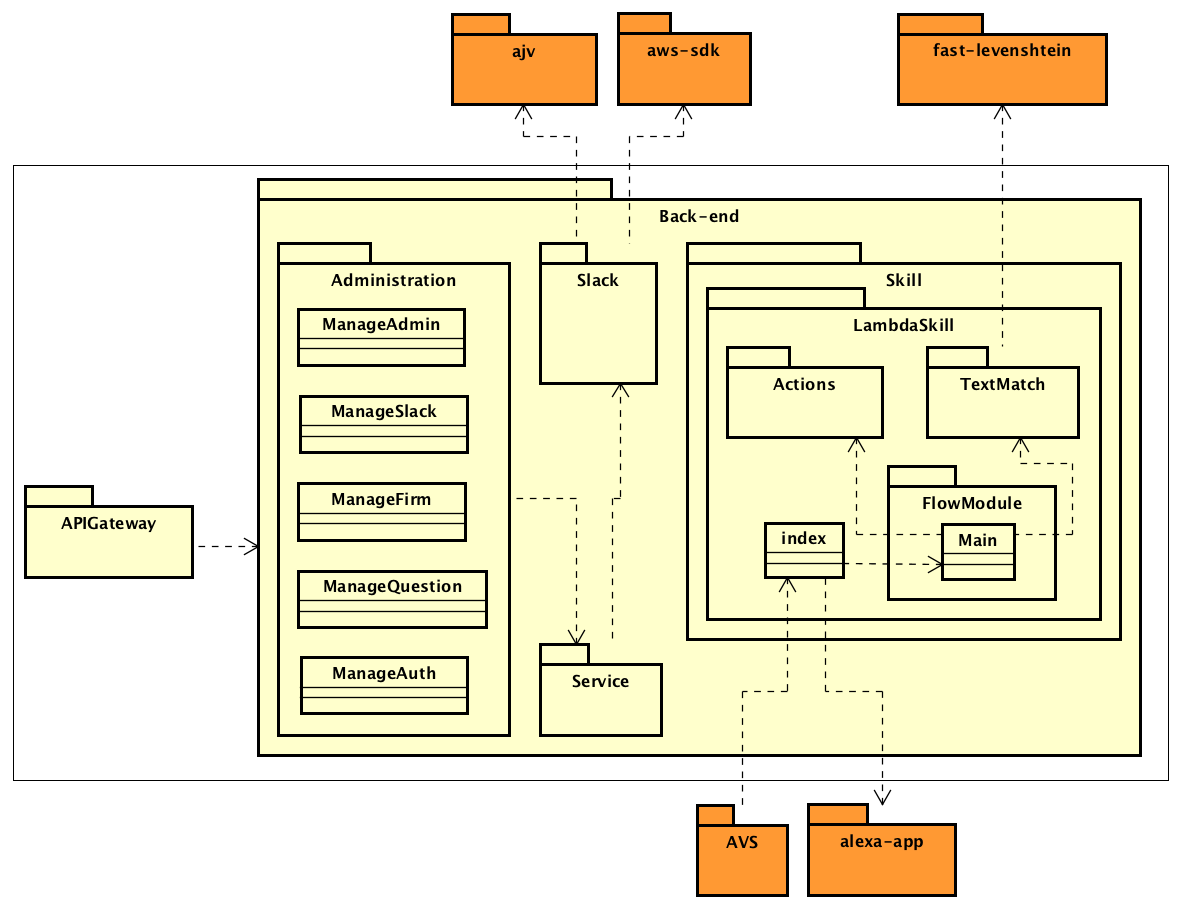
\includegraphics[scale=0.3]{Architettura/Back-end.png}
	\caption{Schema del componente \texttt{Back-End}}
\end{figure}
\subparagraph{Informazioni sul package}
\begin{itemize}
	\item \textbf{Descrizione} Package che contiene tutti i package dedicati alla parte logica dell'applicazione
	\item \textbf{Package contenuti}
	      \begin{itemize}
	      	\item Back-End :: Administration: Package che contiene tutte le funzionalità che un Admin ed un SuperAdmin possono avere;
	      	\item Back-End :: Service: Package che gestisce tutti i servizi disponibili nell'applicazione;
	      	\item Back-End :: Slack: package per la gestione di Slack;
	      	\item Back-End :: Skill: package per la SKill di Alexa.
	      \end{itemize}
\end{itemize}

\subsection{Back-End :: Administration}
\subparagraph{Descrizione} Package che contiene le possibili metodi delegati alla risposta alle interazioni del Front-End.\\
La classe contenuta in questo package non è ancora stata ben definita, poiché un inserimento più ampio di azioni è previsto come requisito opzionale, quindi la definizione specifica di questa classe viene rimandata dopo la codifica dei requisiti obbligatori.

\subsubsection{Back-End :: Administration :: ManageAuth :: index}
\subparagraph{Descrizione} Classe handler per la gestione dell'autenticazione.
\subparagraph{Dipendenze}
\begin{itemize}
	\item \texttt{Back-End :: Service :: AuthService}
	\item	\texttt{Back-End :: Service :: AdminService}
\end{itemize}
\subparagraph{Padre}
\begin{itemize}
	\item	\texttt{Back-End :: Service :: AdminService}
\end{itemize}
\subparagraph{Metodi}
\begin{itemize}
	\item \texttt{action}
	      \subparagraph{Descrizione} Funzione che mediante uno switch dovrà suddividere le azioni da svolgere a seconda delle risorse richieste e metodi utilizzati per la chiamata alle API, da consultare le precedenti tabelle.
	\item \texttt{done}
	      \subparagraph{Descrizione} Funzione che se "err" è null richiama la callback tornando un API trame. In caso di errore verrà impostato la risposta http a 400, in caso contrario a 200.
	      \subparagraph{Parametri}
	      \begin{itemize}
	      	\item \texttt{err : object}contiene l'errore {Error:"",TypeError:""} se avvenuto, null altrimenti;
	      	\item \texttt{res : object}contiene il risultato se l'operazione è riuscita, null altrimenti;
	      \end{itemize}
	\item \texttt{handler}
	      \begin{itemize}
	      	\item \texttt{event : object} evento dell'APIGateway;
	      	\item \texttt{context : object} contesto di chiamata della funzione;
	      	\item \texttt{callback : function} funzione di chiusura chiamata API da richiamare alla fine passando come parametro la risposta.
	      \end{itemize}
\end{itemize}

\subsubsection{Back-End :: Administration :: ManageFirm :: index}
\subparagraph{Descrizione} Classe handler per la gestione delle informazioni sulle aziende e gli ospiti.
\subparagraph{Dipendenze}
\begin{itemize}
	\item \texttt{Back-End :: Service :: FirmService}
\end{itemize}
\subparagraph{Padre}
\begin{itemize}
	\item \texttt{Back-End :: Administration :: ManageFirm}
\end{itemize}
\subparagraph{Metodi}
\begin{itemize}
	\item \texttt{action}
	      \subparagraph{Descrizione} Funzione che mediante uno switch dovrà suddividere le azioni da svolgere a seconda delle risorse richieste e metodi utilizzati per la chiamata alle API, da consultare le precedenti tabelle.
	\item \texttt{done}
	      \subparagraph{Descrizione} Funzione che se "err" è null richiama la callback tornando un API trame. In caso di errore verrà impostato la risposta http a 400, in caso contrario a 200.
	      \subparagraph{Parametri}
	      \begin{itemize}
	      	\item \texttt{err : object}contiene l'errore {Error:"",TypeError:""} se avvenuto, null altrimenti;
	      	\item \texttt{res : object}contiene il risultato se l'operazione è riuscita, null altrimenti;
	      \end{itemize}
	\item \texttt{handler}
	      \begin{itemize}
	      	\item \texttt{event : object} evento dell'APIGateway;
	      	\item \texttt{context : object} contesto di chiamata della funzione;
	      	\item \texttt{callback : function} funzione di chiusura chiamata API da richiamare alla fine passando come parametro la risposta.
	      \end{itemize}
\end{itemize}

\subsubsection{Back-End :: Administration :: ManageQuestion :: index}
\subparagraph{Descrizione} Classe handler per la gestione delle domande e delle risposte.
\subparagraph{Dipendenze}
\begin{itemize}
	\item \texttt{Back-End :: Service :: QuestionService}
\end{itemize}
\subparagraph{Padre}
\begin{itemize}
	\item \texttt{Back-End :: Administration :: ManageQuestion}
\end{itemize}
\subparagraph{Metodi}
\begin{itemize}
	\item \texttt{action}
	      \subparagraph{Descrizione} Funzione che mediante uno switch dovrà suddividere le azioni da svolgere a seconda delle risorse richieste e metodi utilizzati per la chiamata alle API, da consultare le precedenti tabelle.
	\item \texttt{done}
	      \subparagraph{Descrizione} Funzione che se "err" è null richiama la callback tornando un API trame. In caso di errore verrà impostato la risposta http a 400, in caso contrario a 200.
	      \subparagraph{Parametri}
	      \begin{itemize}
	      	\item \texttt{err : object}contiene l'errore {Error:"",TypeError:""} se avvenuto, null altrimenti;
	      	\item \texttt{res : object}contiene il risultato se l'operazione è riuscita, null altrimenti;
	      \end{itemize}
	\item \texttt{handler}
	      \begin{itemize}
	      	\item \texttt{event : object} evento dell'APIGateway;
	      	\item \texttt{context : object} contesto di chiamata della funzione;
	      	\item \texttt{callback : function} funzione di chiusura chiamata API da richiamare alla fine passando come parametro la risposta.
	      \end{itemize}
\end{itemize}

\subsubsection{Back-End :: Administration :: ManageSlack :: index}
\subparagraph{Descrizione} Classe handler per la gestione delle impostazioni dell'integrazione con Slack.
\subparagraph{Dipendenze}
\begin{itemize}
	\item \texttt{Back-End :: Service :: SlackService :: InfoSlack}
\end{itemize}
\subparagraph{Padre}
\begin{itemize}
	\item \texttt{Back-End :: Administration :: ManageSlack}
\end{itemize}
\subparagraph{Metodi}
\begin{itemize}
	\item \texttt{action}
	      \subparagraph{Descrizione} Funzione che mediante uno switch dovrà suddividere le azioni da svolgere a seconda delle risorse richieste e metodi utilizzati per la chiamata alle API, da consultare le precedenti tabelle.
	\item \texttt{done}
	      \subparagraph{Descrizione} Funzione che se "err" è null richiama la callback tornando un API trame. In caso di errore verrà impostato la risposta http a 400, in caso contrario a 200.
	      \subparagraph{Parametri}
	      \begin{itemize}
	      	\item \texttt{err : object}contiene l'errore {Error:"",TypeError:""} se avvenuto, null altrimenti;
	      	\item \texttt{res : object}contiene il risultato se l'operazione è riuscita, null altrimenti;
	      \end{itemize}
	\item \texttt{handler}
	      \begin{itemize}
	      	\item \texttt{event : object} evento dell'APIGateway;
	      	\item \texttt{context : object} contesto di chiamata della funzione;
	      	\item \texttt{callback : function} funzione di chiusura chiamata API da richiamare alla fine passando come parametro la risposta.
	      \end{itemize}
\end{itemize}

\subsection{Back-End :: Service :: AuthService :: AuthService}
\begin{figure}[!h]
	\centering
	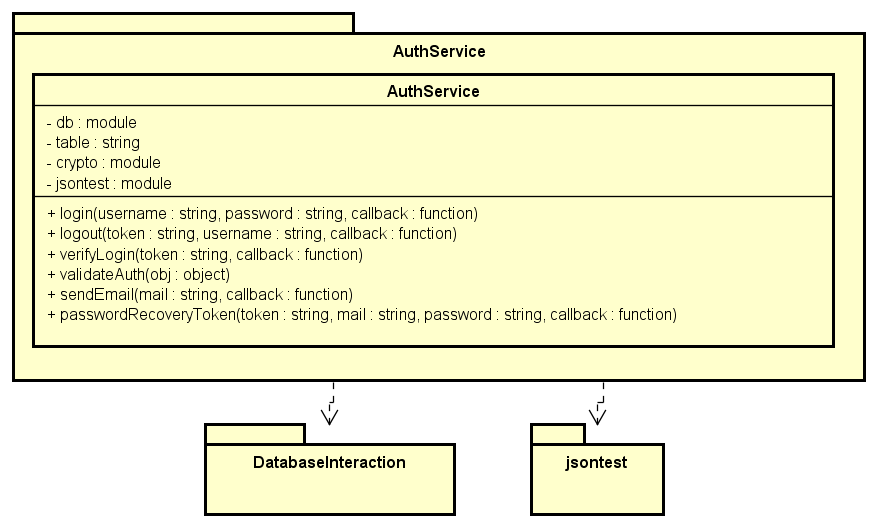
\includegraphics[scale=0.6]{Architettura/Back-End/Service/AuthService.png}
	\caption{Schema del componente \texttt{Back-End :: Service :: AuthService}}
\end{figure}
\subparagraph{Descrizione} Modulo che fornisce i metodi per l'autenticazione degli amministratori.
\subparagraph{Dipendenze}
\begin{itemize}
	\item \texttt{Back-End :: Service :: DatabaseInteraction}
	\item \texttt{Back-End :: Service :: TestJson}
\end{itemize}
\subparagraph{Padre}
\begin{itemize}
	\item \texttt{Back-End :: Service :: AuthService}
\end{itemize}
\subparagraph{Metodi}
\begin{itemize}
	\item \texttt{Login}
	      \subparagraph{Descrizione} funzione che passa a callback (err,res) e in res l'amministratore con quel username e password
	      \subparagraph{Parametri}
	      \begin{itemize}
	      	\item \texttt{username : string}
	      	\item \texttt{password : string}
	      	\item \texttt{callback : function}
	      \end{itemize}
	\item \texttt{Logout} funzione che passa a callback (err,res) res sarà sempre null, e cancella il token dall'utente
	      \subparagraph{Descrizione} Funzione per il login
	      \subparagraph{Parametri}
	      \begin{itemize}
	      	\item \texttt{token : string}
	      	\item \texttt{username : string}
	      	\item \texttt{callback : function}
	      \end{itemize}
	\item \texttt{verifyLogin} funzione che passa a callback (err,res) e in res l'amministratore possedente il token
	      \subparagraph{Descrizione} Funzione per il login
	      \subparagraph{Parametri}
	      \begin{itemize}
	      	\item \texttt{token : string}
	      	\item \texttt{callback : function}
	      \end{itemize}
	\item \texttt{passwordRecoveryToken} funzione che passa a callback (err,res)
	      \subparagraph{Descrizione} Funzione per il login
	      \subparagraph{Parametri} \begin{itemize}
	\item \texttt{mail : string}
	\item \texttt{callback : function}
\end{itemize}
\item \texttt{validateAuth} ritorna un {"validate":"","error":[]} e verifica l'attinenza al JSONSchema dell'oggetto Auth.
\subparagraph{Descrizione} Funzione per il login
\subparagraph{Parametri} \begin{itemize}
\item \texttt{obj : object}
\end{itemize}
\item \texttt{sendEmail} funzione che passa a callback (err,res)
\subparagraph{Descrizione} Funzione per il login
\subparagraph{Parametri} \begin{itemize}
\item \texttt{token : string}
\item \texttt{callback : function}
\end{itemize}
\end{itemize}


\subsection{Back-End :: Service :: AdminService :: AdminService}
\begin{figure}[!h]
	\centering
	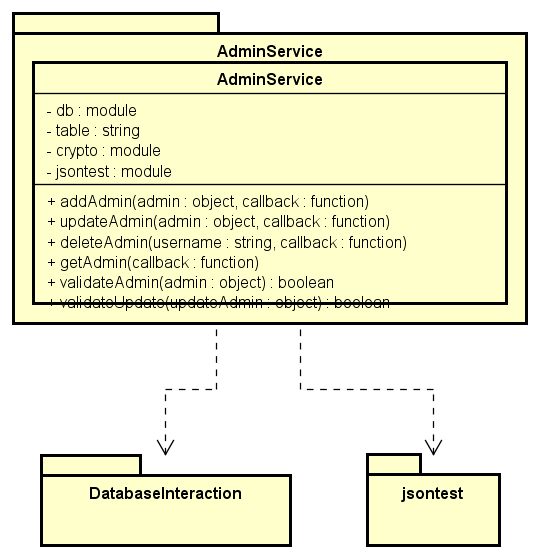
\includegraphics[scale=0.6]{Architettura/Back-End/Service/AdminService.png}
	\caption{Schema del componente \texttt{Back-End :: Service :: AdminService}}
\end{figure}
\subparagraph{Descrizione} Modulo contenente i servizi rivolti all'admin
\subparagraph{Dipendenze}
\begin{itemize}
	\item \texttt{Back-End :: Service :: DatabaseInteraction}
	\item \texttt{Back-End :: Service :: TestJson}
\end{itemize}
\subparagraph{Costanti}
\begin{itemize}
	\item \texttt{Back-End :: Service :: AdminService}
\end{itemize}
\subparagraph{Metodi}\begin{itemize}
\item \texttt{addAdmin}
\subparagraph{Descrizione} funzione che inserisce nel database Admin. Passa a callback (err,res) e in res l'amministratore con quel username e password
\subparagraph{Parametri} \begin{itemize}
\item \texttt{admin : object}
\item \texttt{callback : function}
\end{itemize}
\item \texttt{updateAdmin}
\subparagraph{Descrizione} funzione che aggiorna nel database l'admin. Passa a callback (err,res) e in res contiene null.
\subparagraph{Parametri} \begin{itemize}
\item \texttt{admin : object}
\item \texttt{callback : function}
\end{itemize}
\item \texttt{deleteAdmin}
\subparagraph{Descrizione} funzione cancella l'amministratore passato dal database. Passa a callback (err,res) e in res null
\subparagraph{Parametri} \begin{itemize}
\item \texttt{username : string}
\item \texttt{callback : function}
\end{itemize}
\item \texttt{getAdmin}
\subparagraph{Descrizione} funzione che passa a callback (err,res) e in res tutti gli amministratori.
\subparagraph{Parametri} \begin{itemize}
\item \texttt{callback : function}
\end{itemize}
\item \texttt{validateAdmin}
\subparagraph{Descrizione} ritorna un {"validate":"","error":[]} e verifica l'attinenza al JSONSchema dell'oggetto admin.
\subparagraph{Parametri} \begin{itemize}
\item \texttt{admin : object}
\end{itemize}
\item \texttt{validateUpdate}
\subparagraph{Descrizione} ritorna un {"validate":"","error":[]} e verifica l'attinenza al JSONSchema dell'oggetto update.
\subparagraph{Parametri} \begin{itemize}
\item \texttt{updateAdmin : object}
\end{itemize}
\end{itemize}

\subsection{Back-End :: Service :: SlackService :: InfoSlack}
\begin{figure}[!h]
	\centering
	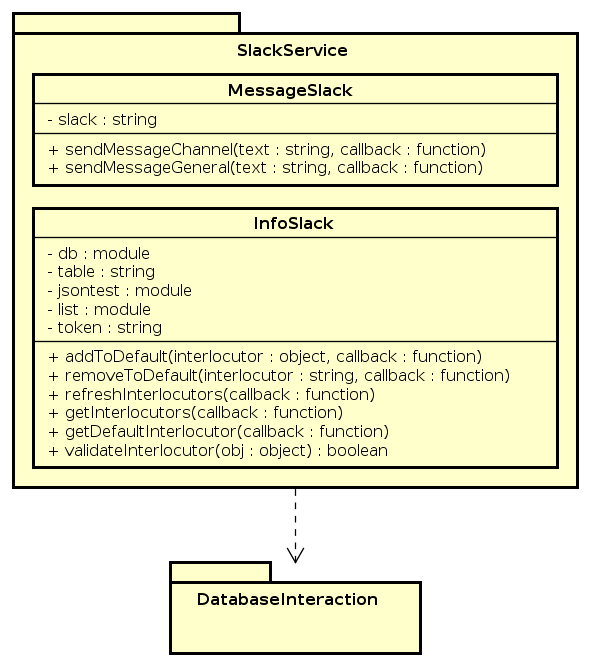
\includegraphics[scale=0.6]{Architettura/Back-End/Service/SlackService.png}
	\caption{Schema del componente \texttt{Back-End :: Service :: SlackService}}
\end{figure}
\subparagraph{Descrizione} Modulo contenente i servizi rivolti all'admin
\subparagraph{Dipendenze}
\begin{itemize}
	\item \texttt{Back-End :: Service :: DatabaseInteraction}
	\item \texttt{Back-End :: Service :: TestJson}
	\item \texttt{Back-End :: Slack :: Slack}
\end{itemize}
\subparagraph{Padre}
\begin{itemize}
	\item \texttt{Back-End :: Service :: SlackService}
\end{itemize}
\subparagraph{Metodi}\begin{itemize}
\item \texttt{addToDefault}
\subparagraph{Descrizione} funzione che modifica l'interlocutor nel database impostando isDefault a false. Passa a callback (err,res) e in res null
\subparagraph{Parametri} \begin{itemize}
\item \texttt{interlocutor : object}
\item \texttt{callback : function}
\end{itemize}
\item \texttt{removeToDefault}
\subparagraph{Descrizione} funzione che modifica l'interlocutor nel database impostando isDefault a false. Passa a callback (err,res) e in res null
\subparagraph{Parametri} \begin{itemize}
\item \texttt{interlocutor : object}
\item \texttt{callback : function}
\end{itemize}
\item \texttt{refreshInterlocutors}
\subparagraph{Descrizione} funzione che sincronizza gli interlocutor tra il team di Slack senza perdere le caratteristiche già presenti. Passa a callback (err,res) e in res null
\subparagraph{Parametri} \begin{itemize}
\item \texttt{callback : function}
\end{itemize}
\item \texttt{getInterlocutors}
\subparagraph{Descrizione} funzione che passa a callback (err,res) e in res la lista degli interlocutori presenti nel database.
\subparagraph{Parametri} \begin{itemize}
\item \texttt{callback : function}
\end{itemize}
\item \texttt{getDefaultInterlocutors}
\subparagraph{Descrizione} funzione che passa a callback (err,res) e in res la lista degli interlocutori con isDefault impostato a "true" presenti nel database.
\subparagraph{Parametri} \begin{itemize}
\item \texttt{callback : function}
\end{itemize}
\item \texttt{validateInterlocutor}
\subparagraph{Descrizione} ritorna un {"validate":"","error":[]} e verifica l'attinenza al JSONSchema dell'oggetto interlocutor.
\subparagraph{Parametri} \begin{itemize}
\item \texttt{obj : object}
\end{itemize}
\end{itemize}

\subsection{Back-End :: Service :: SlackService :: MessageSlack}
\begin{figure}[!h]
	\centering
	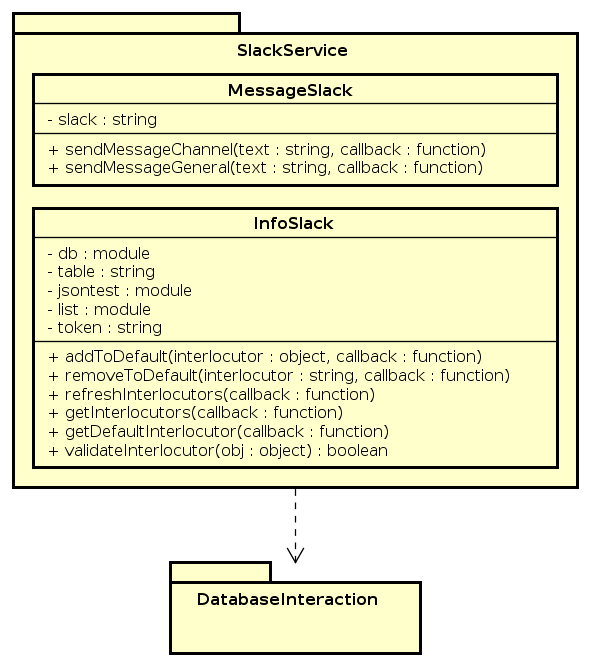
\includegraphics[scale=0.6]{Architettura/Back-End/Service/SlackService.png}
	\caption{Schema del componente \texttt{Back-End :: Service :: SlackService}}
\end{figure}
\subparagraph{Descrizione} Modulo contenente i servizi rivolti all'admin
\subparagraph{Dipendenze}
\begin{itemize}
	\item \texttt{Back-End :: Slack :: Slack}
\end{itemize}
\subparagraph{Padre}
\begin{itemize}
	\item \texttt{Back-End :: Service :: SlackService}
\end{itemize}
\subparagraph{Metodi}\begin{itemize}
\item \texttt{SendMessageChannel}
\subparagraph{Descrizione} funzione che spedisce un messaggio contenente text in channel. Passa a callback (err,res) e in res null
\subparagraph{Parametri} \begin{itemize}
\item \texttt{text : string}
\item \texttt{channel : string}
\item \texttt{callback : function}
\end{itemize}
\item \texttt{SendMessageGeneral}
\subparagraph{Descrizione} funzione che spedisce un messaggio contenente text in general. Passa a callback (err,res) e in res null
\subparagraph{Parametri} \begin{itemize}
\item \texttt{text : string}
\item \texttt{callback : function}
\end{itemize}
\end{itemize}


\subsection{Back-End :: Service :: FirmService :: FirmService}
\begin{figure}[!h]
	\centering
	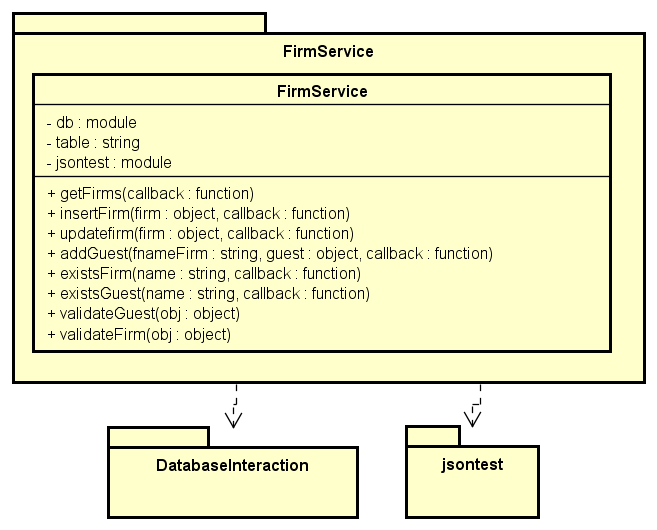
\includegraphics[scale=0.6]{Architettura/Back-End/Service/FirmService.png}
	\caption{Schema del componente \texttt{Back-End :: Service :: FirmService}}
\end{figure}
\subparagraph{Descrizione} Modulo contenente i servizi rivolti all'admin
\subparagraph{Dipendenze}
\begin{itemize}
	\item \texttt{Back-End :: Service :: DatabaseInteraction}
	\item \texttt{Back-End :: Service :: TestJson}
\end{itemize}
\subparagraph{Padre}
\begin{itemize}
	\item \texttt{Back-End :: Service :: FirmService}
\end{itemize}
\subparagraph{Metodi}\begin{itemize}
\item \texttt{getFirms}
\subparagraph{Descrizione} funzione che passa a callback (err,res) e in res la lista delle firm contenute nel database
\subparagraph{Parametri} \begin{itemize}
\item \texttt{callback : function}
\end{itemize}
\item \texttt{inserFirm}
\subparagraph{Descrizione} funzione che inserisce l'oggetto firm nel database. Passa a callback (err,res) e in res null
\subparagraph{Parametri} \begin{itemize}
\item \texttt{interlocutor : object}
\item \texttt{callback : function}
\end{itemize}
\item \texttt{updateFirm}
\subparagraph{Descrizione} funzione che aggiorna l'oggetto firm nel database. Passa a callback (err,res) e in res null
\subparagraph{Parametri} \begin{itemize}
\item \texttt{firm : object}
\item \texttt{callback : function}
\end{itemize}
\item \texttt{addGuest}
\subparagraph{Descrizione} :funzione che aggiunge l'oggetto guest sulla corrispettiva azienda nel database. Passa a callback (err,res) e in res null
\subparagraph{Parametri} \begin{itemize}
\item \texttt{nameFirm : string}
\item \texttt{guest : object}
\item \texttt{callback : function}
\end{itemize}
\item \texttt{existsFirm}
\subparagraph{Descrizione} :funzione che verifica l'esistenza dell'oggetto firm nel database. Passa a callback (err,res) e in res un booleano
\subparagraph{Parametri} \begin{itemize}
\item \texttt{name : string}
\item \texttt{callback : function}
\end{itemize}
\item \texttt{existsGuest}
\subparagraph{Descrizione} funzione che verifica l'esistenza dell'oggetto guest nel database. Passa a callback (err,res) e in res un booleano
\subparagraph{Parametri} \begin{itemize}
\item \texttt{name : string}
\item \texttt{callback : function}
\end{itemize}
\item \texttt{validateGuest}
\subparagraph{Descrizione} ritorna un oggetto {"validate":"","error":[]} e verifica l'attinenza al JSONSchema dell'oggetto Guest.
\subparagraph{Parametri} \begin{itemize}
\item \texttt{obj : object}
\end{itemize}
\item \texttt{validateFirm}
\subparagraph{Descrizione} ritorna un {"validate":"","error":[]}  e verifica l'attinenza al JSONSchema dell'oggetto Firm.
\subparagraph{Parametri} \begin{itemize}
\item \texttt{obj : object}
\end{itemize}
\end{itemize}

\subsection{Back-End :: Service :: QuestionService :: QuestionService}
\begin{figure}[!h]
	\centering
	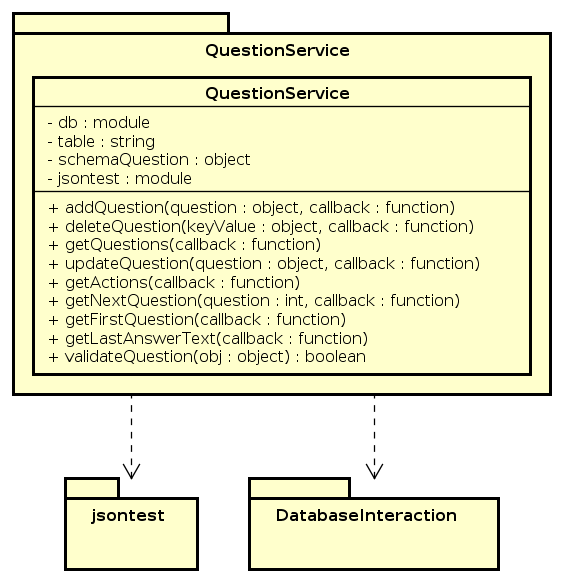
\includegraphics[scale=0.6]{Architettura/Back-End/Service/QuestionService.png}
	\caption{Schema del componente \texttt{Back-End :: Service :: QuestionService}}
\end{figure}
\subparagraph{Descrizione} Modulo contenente i servizi rivolti all'admin
\subparagraph{Dipendenze}
\begin{itemize}
	\item \texttt{Back-End :: Service :: DatabaseInteraction}
	\item \texttt{Back-End :: Service :: TestJson}
\end{itemize}
\subparagraph{Padre}
\begin{itemize}
	\item \texttt{Back-End :: Service :: QuestionService}
\end{itemize}
\subparagraph{Metodi}\begin{itemize}
\item \texttt{getQuestions}
\subparagraph{Descrizione}funzione che passa a callback (err,res) e in res la lista delle question contenute nel database
\subparagraph{Parametri}
\begin{itemize}
	\item \texttt{callback : function}
\end{itemize}
\item \texttt{addQuestion}
\subparagraph{Descrizione}funzione che inserisce l'oggetto firm nel database. Passa a callback (err,res) e in res null
\subparagraph{Parametri}
\begin{itemize}
	\item \texttt{question : object}
	\item \texttt{callback : function}
\end{itemize}
\item \texttt{deleteQuestion}
\subparagraph{Descrizione}funzione che elimina l'oggetto firm nel database. Passa a callback (err,res) e in res null
\subparagraph{Parametri}
\begin{itemize}
	\item \texttt{keyValue : object}
	\item \texttt{callback : function}
\end{itemize}
\item \texttt{updateQuestion}
\subparagraph{Descrizione}funzione che inserisce l'oggetto firm nel database. Passa a callback (err,res) e in res null
\subparagraph{Parametri}
\begin{itemize}
	\item \texttt{question : object}
	\item \texttt{callback : function}
\end{itemize}
\item \texttt{getActions}
\subparagraph{Descrizione}funzione che passa a callback (err,res) e in res la lista delle Action contenute nel database
\subparagraph{Parametri}
\begin{itemize}
	\item \texttt{callback : function}
\end{itemize}
\item \texttt{getNextQuestions}
\subparagraph{Descrizione}funzione che passa a callback (err,res) e in res la  question successiva contenuta nel database rispetto a quella di chiave "question"
\subparagraph{Parametri}
\begin{itemize}
	\item \texttt{question : int}
	\item \texttt{callback : function}
\end{itemize}
\item \texttt{getFirstQuestions}
\subparagraph{Descrizione}funzione che passa a callback (err,res) e in res l'ultima question contenute nel database
\subparagraph{Parametri}
\begin{itemize}
	\item \texttt{callback : function}
\end{itemize}
\item \texttt{validateQuestion}
\subparagraph{Descrizione}ritorna un {"validate":"","error":[]}  e verifica l'attinenza al JSONSchema dell'oggetto Question.
\subparagraph{Parametri}
\begin{itemize}
	\item \texttt{obj : object}
\end{itemize}
\end{itemize}

\subsection{Back-End :: Service :: LogService :: LogService}
\begin{figure}[!h]
	\centering
	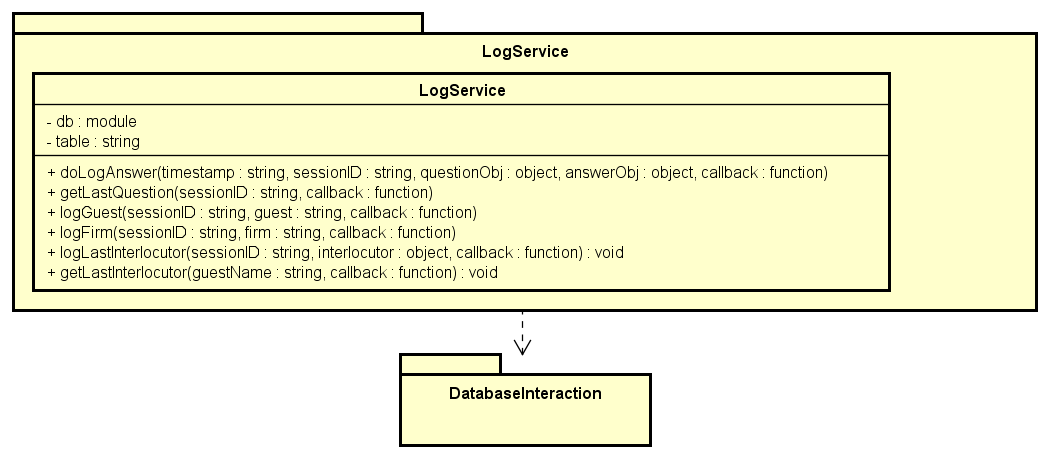
\includegraphics[scale=0.6]{Architettura/Back-End/Service/LogService.png}
	\caption{Schema del componente \texttt{Back-End :: Service :: LogService}}
\end{figure}
\subparagraph{Descrizione} Modulo contenente i servizi rivolti al loggin della conversazione
\subparagraph{Dipendenze}
\begin{itemize}
	\item \texttt{Back-End :: Service :: DatabaseInteraction}
\end{itemize}
\subparagraph{Costanti}
\begin{itemize}
	\item \texttt{Back-End :: Service :: LogService}
\end{itemize}
\subparagraph{Metodi}\begin{itemize}
\item \texttt{doLogAnswer}
\subparagraph{Descrizione}funzione inserisce nel database l'oggetto Questionobj e QuestionAnswer incapsulati in un oggetto contenente una lista della conversazione "logg" e il sessionID. Passa a callback (err,res) e in res null
\subparagraph{Parametri}
\begin{itemize}
	\item \texttt{timestamp : string}
	\item \texttt{sessionID : string}
	\item \texttt{questionObj : object}
	\item \texttt{questionObj : object}
	\item \texttt{callback : function}
\end{itemize}
\end{itemize}

\subsection{Back-End :: Service :: DatabaseInteraction :: DatabaseInteraction}
\begin{figure}[!h]
	\centering
	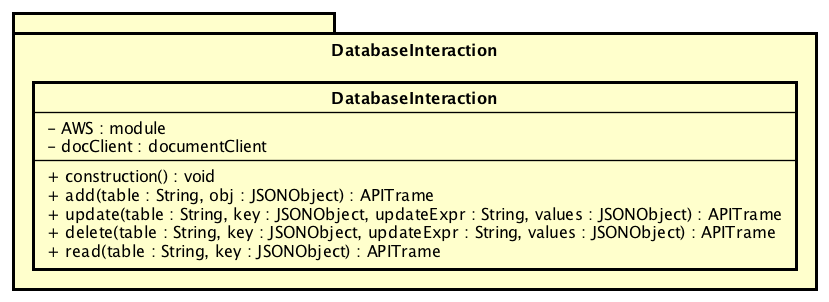
\includegraphics[scale=0.5]{Architettura/Back-End/Service/DatabaseInteraction.png}
	\caption{Schema del componente \texttt{Back-End :: Service :: DatabaseInteraction}}
\end{figure}
\subparagraph{Descrizione} Modulo contenente i servizi rivolti x loggin della conversazione
\subparagraph{Dipendenze}
\begin{itemize}
	\item \texttt{AWS-sdk}
\end{itemize}
\subparagraph{Padre}
\begin{itemize}
	\item \texttt{Back-End :: Service :: DatabaseInteraction}
\end{itemize}
\subparagraph{Metodi}\begin{itemize}
\item \texttt{insert}
\subparagraph{Descrizione} Inserisce l'oggetto nella "table" di dynamo attraverso le sdk e ci passa callback.
\subparagraph{Parametri}
\begin{itemize}
	\item \texttt{table : string}
	\item \texttt{sessionID : object}
	\item \texttt{callback : function}
\end{itemize}
\item \texttt{update}
\subparagraph{Descrizione} Aggiorna l'oggetto con chiave "key" nella "table" di dynamo attraverso le sdk e ci passa callback.
\subparagraph{Parametri}
\begin{itemize}
	\item \texttt{table : string}
	\item \texttt{key : object}
	\item \texttt{updateExpression : string}
	\item \texttt{replace : object}
	\item \texttt{callback : function}
\end{itemize}

\item \texttt{remove}
\subparagraph{Descrizione} rimuove l'oggetto con chiave "key" nella "table" di dynamo attraverso le sdk e ci passa callback.
\subparagraph{Parametri}
\begin{itemize}
	\item \texttt{table : string}
	\item \texttt{key : object}
	\item \texttt{callback : function}
\end{itemize}

\item \texttt{read}
\subparagraph{Descrizione} Esegue la lettura dell'oggetto con chiave "key" nella "table" di dynamo attraverso le sdk e ci passa callback.
\subparagraph{Parametri}
\begin{itemize}
	\item \texttt{table : string}
	\item \texttt{key : object}
	\item \texttt{callback : function}
\end{itemize}

\item \texttt{query}
\subparagraph{Descrizione} Esegue la lettura delle "proprieties" di tutti gli oggetti rispettanti la filter expression con i valori "attribute value" nella "table" di dynamo attraverso le sdk e ci passa callback.
\subparagraph{Parametri}
\begin{itemize}
	\item \texttt{table : string}
	\item \texttt{proprieties : string}
	\item \texttt{filterExpression : string}
	\item \texttt{ExpressionAttributeValue : object}
	\item \texttt{callback : function}
\end{itemize}
\end{itemize}

\subsection{Back-End :: Service :: JsonTest :: TestJson}
\subparagraph{Descrizione} Modulo contenente i servizi rivolti alla validazione di un oggetto rispettivamente ad un JSONSchema.
\subparagraph{Dipendenze}
\begin{itemize}
	\item \texttt{Ajv.js}
\end{itemize}
\subparagraph{Padre}
\begin{itemize}
	\item \texttt{Back-End :: Service :: JsonTest}
\end{itemize}
\subparagraph{Metodi}\begin{itemize}
\item \texttt{test}
\subparagraph{Descrizione} Controlla l'attinenza dell'oggetto obj allo JSONSchema utilizzando la libreria Ajv e tornando {"valid":false,"errors":array} in caso di errore con errors gli errori identificati, {"valid":true} in caso di attinenza.
\subparagraph{Parametri}
\begin{itemize}
	\item \texttt{schema : object}
	\item \texttt{obj : object}
\end{itemize}
\end{itemize}

\newpage
\subsection{Back-End :: Slack}
\begin{figure}[!h]
	\centering
	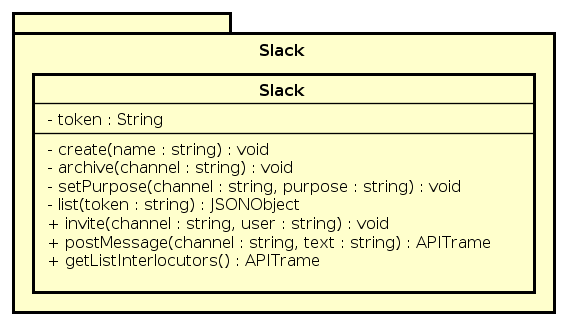
\includegraphics[scale=0.6]{Architettura/Back-End/Slack.png}
	\caption{Schema del componente \texttt{Back-End :: Slack}}
\end{figure}
\subparagraph{Descrizione} Package che contiene le possibili metodi delegati alla risposta alle interazioni del Front-End.\\
La classe contenuta in questo package non è ancora stata ben definita, poiché un inserimento più ampio di azioni è previsto come requisito opzionale, quindi la definizione specifica di questa classe viene rimandata dopo la codifica dei requisiti obbligatori.
\subparagraph{Lista dei Metodi}
\begin{itemize}
\item \texttt{Back-End :: Slack :: createChannel}
\item \texttt{Back-End :: Slack :: channelList}
\item \texttt{Back-End :: Slack :: invite}
\item \texttt{Back-End :: Slack :: NameID}
\item \texttt{Back-End :: Slack :: setPurpose}
\item \texttt{Back-End :: Slack :: unarchive}
\item \texttt{Back-End :: Slack :: userList}
\item \texttt{Back-End :: Slack :: postMessage}
\end{itemize}

\subsubsection{Back-End :: Slack :: postMessage}
\subparagraph{Descrizione} Modulo per inviare messaggi ad un canale Slack
\subparagraph{Dipendenze}
\begin{itemize}
	\item \texttt{https};
	\item \texttt{querystring};
	\item \texttt{Back-End :: Slack :: ChannelList};
	\item \texttt{Back-End :: Slack :: createChannel};
	\item \texttt{Back-End :: Slack :: NameID};
	\item \texttt{Back-End :: Slack :: unarchive};
	\item \texttt{Back-End :: Slack :: invite};
	\item \texttt{Back-End :: Slack :: setPurpose}.
\end{itemize}
\subparagraph{Padre}
\begin{itemize}
	\item \texttt{Back-End :: Slack}.
\end{itemize}
\subparagraph{Metodi}
\begin{itemize}
	\item \texttt{postMessage}
	      \subparagraph{Descrizione} Metodo per inviare un messaggio ad un dato canale. Se il canale non esiste viene creato e vengono invitati gli utenti di default impostati dagli amministratori. Se il canale è archiviato questo viene disarchiviato e vengono invitati gli utenti di default.
	      \subparagraph{Parametri}
	      \begin{itemize}
	      	\item \texttt{token};
	      	\item \texttt{channelName};
	      	\item \texttt{text};
	      	\item \texttt{callback}.
	      \end{itemize}
	      \subparagraph{Ritorno} Utilizzando la callback, il metodo restituisce l'ID dell'utente o un errore.
\end{itemize}

\subsection{Back-End :: Skill :: index}
\subparagraph{Descrizione} Modulo per ottenere la lista degli utenti di Slack
\subparagraph{Dipendenze}
\begin{itemize}
	\item \texttt{Back-End :: Skill :: LambdaSkill};
	\item \texttt{alexa-app}.
\end{itemize}
\subparagraph{Padre}
\begin{itemize}
	\item \texttt{Back-End :: Skill}
\end{itemize}
\subparagraph{Metodi}
\begin{itemize}
	\item \texttt{app.launch}
	      \subparagraph{Descrizione} Handler per le chiamate alla Skill con intent Launch.
	      \subparagraph{Parametri}
	      \begin{itemize}
	      	\item \texttt{callback}.
	      \end{itemize}
	      \subparagraph{Ritorno} Utilizzando la callback, il metodo ottiene i dati della richiesta mandata da Alexa e crea l'oggetto risposta che verrà restituito in callback.
	\item \texttt{app.intent}
	      \subparagraph{Descrizione} Handler per le chiamate alla Skill con intent custom.
	      \subparagraph{Parametri}
	      \begin{itemize}
	      	\item \texttt{intentName};
	      	\item \texttt{intentConfiguration};
	      	\item \texttt{callback}.
	      \end{itemize}
	      \subparagraph{Ritorno} Utilizzando la callback, il metodo ottiene i dati della richiesta mandata da Alexa e crea l'oggetto risposta che verrà restituito in callback.
	\item \texttt{app.sessionEnded}
	      \subparagraph{Descrizione} Handler per le chiamate alla Skill con intent ended.
	      \subparagraph{Parametri}
	      \begin{itemize}
	      	\item \texttt{callback}.
	      \end{itemize}
	      \subparagraph{Ritorno} Utilizzando la callback, il metodo ottiene i dati della richiesta mandata da Alexa e crea l'oggetto risposta che verrà restituito in callback.
	\item \texttt{app.utterances}
	      \subparagraph{Descrizione} Ridefinizione del metodo per la generazione delle utterances.
	      \subparagraph{Ritorno} Il metodo ritorna una stringa di utterances espansa.
\end{itemize}

\subsection{Back-End :: Skill :: LambdaSkill :: Main}
\subparagraph{Descrizione} Modulo per la gestione della logica della skill.
\subparagraph{Dipendenze}
\begin{itemize}
	\item \texttt{Back-End :: Skill :: LambdaSkill :: FlowModule :: FlowModule}
\end{itemize}
\subparagraph{Padre}
\begin{itemize}
	\item \texttt{Back-End :: Skill :: LambdaSkill}
\end{itemize}
\subparagraph{Metodi}
\begin{itemize}
	\item \texttt{main}
	      \subparagraph{Descrizione} Metodo che gestisce la chiamata alla routine di azioni da eseguire quando l'AV riceve una risposta da parte di Alexa.
	      \subparagraph{Parametri}
	      \begin{itemize}
	      	\item \texttt{textAnswer};
	      	\item \texttt{sessionId};
	      	\item \texttt{session};
	      	\item \texttt{callback}.
	      \end{itemize}
	      \subparagraph{Ritorno} Il metodo restituisce in callback il testo della risposta dell'AV.
\end{itemize}

\subsection{Back-End :: Skill :: LambdaSkill :: TextMatch :: TextMatch}
\subparagraph{Descrizione} Package che rende disponibili i metodi matching del testo di una risposta con un array di possibili testi.
\subparagraph{Dipendenze} 
\begin{itemize}
\item \texttt{fast-levenshtein}
\end{itemize}
\subparagraph{Padre} 
\begin{itemize}
\item \texttt{Back-End :: Skill :: LambdaSkill :: TextMatch}
\end{itemize}
\subparagraph{Metodi}
\begin{itemize}
	\item \texttt{matchText}
	      \subparagraph{Descrizione} Metodo per il match di una stringa di testo con un array di stringhe di testo
	      \subparagraph{Parametri}
	      \begin{itemize}
	      	\item \texttt{textToMatch};
	      	\item \texttt{textsAvailable}.
	      \end{itemize}
	      \subparagraph{Ritorno} Il metodo restituisce il testo più vicino o un errore se troppo distante dai testi disponibili.
\end{itemize}


\subsection{Back-End :: Skill :: LambdaSkill :: FlowModule :: FlowModule}
\subparagraph{Descrizione} Modulo per la gestione logica dell'AV. Si occupa di risposte dell'utente e di formulare le domande.
\subparagraph{Dipendenze}
\begin{itemize}
	\item \texttt{Back-End :: Skill :: LambdaSkill :: TextMatch};
	\item \texttt{Back-End :: Skill :: LambdaSkill :: Actions};
	\item \texttt{Back-End :: Service :: QuestionService};
	\item \texttt{Back-End :: Service :: LogService}.
\end{itemize}
\subparagraph{Padre}
\begin{itemize}
	\item \texttt{Back-End :: Skill :: LambdaSkill :: FlowModule}
\end{itemize}
\subparagraph{Metodi}
\begin{itemize}
	\item \texttt{routine}
	      \subparagraph{Descrizione} Metodo per la l'esecuzione della sequenza di azioni per la comprensione di una risposta e la generazione della domanda seguente
	      \subparagraph{Parametri}
	      \begin{itemize}
	      	\item \texttt{textAnswer};
	      	\item \texttt{sessionId};
	      	\item \texttt{session};
	      	\item \texttt{callback}.
	      \end{itemize}
	      \subparagraph{Ritorno} Il metodo restituisce tramite la callback un oggetto JSON con i dati sulla prossima domanda da porre o un errore.

	\item \texttt{getLastQuestion}
	      \subparagraph{Descrizione} Metodo per ottenere l'ultima domanda posta all'ospite dato il suo session ID.
	      \subparagraph{Parametri}
	      \begin{itemize}
	      	\item \texttt{sessionId};
	      	\item \texttt{session};
	      	\item \texttt{callback}.
	      \end{itemize}
	      \subparagraph{Ritorno} Il metodo restituisce tramite la callback un oggetto JSON contenente l'ultima domanda posta, con le relative risposte associate, oppure un errore.

	\item \texttt{getFirstQuestion}
	      \subparagraph{Descrizione} Metodo per ottenere la prima domanda da porre all'ospite.
	      \subparagraph{Parametri}
	      \begin{itemize}
	      	\item \texttt{callback}.
	      \end{itemize}
	      \subparagraph{Ritorno} Il metodo restituisce tramite la callback un oggetto JSON contenente la prima domanda, con le relative risposte associate, oppure un errore.

	\item \texttt{matchPossibleAnswers}
	      \subparagraph{Descrizione} Metodo per confrontare la risposta rilevata da AVS con le risposte disponibili.
	      \subparagraph{Parametri}
	      \begin{itemize}
	      	\item \texttt{receivedAnswerText};
	      	\item \texttt{questionAsked}.
	      \end{itemize}
	      \subparagraph{Ritorno} Il metodo restituisce l'oggetto answer più vicino alla risposta ricevuta oppure un errore.

	\item \texttt{composeNextQuestion}
	      \subparagraph{Descrizione} Metodo per generare il testo delle domande dell'AV durante la conversazione.
	      \subparagraph{Parametri}
	      \begin{itemize}
	      	\item \texttt{session};
	      	\item \texttt{question}.
	      \end{itemize}
	      \subparagraph{Ritorno} Il metodo restituisce un oggetto JSON con il testo della domanda o un errore.

	\item \texttt{callAction}
	      \subparagraph{Descrizione} Metodo per lanciare l'esecuzione di una action.
	      \subparagraph{Parametri}
	      \begin{itemize}
	      	\item \texttt{actionId};
	      	\item \texttt{actionParameters};
	      	\item \texttt{callback}.
	      \end{itemize}
	      \subparagraph{Ritorno} Il metodo restituisce in callback il risultato dell'esecuzione dell'action o un errore.

	\item \texttt{logAnswerOnDB}
	      \subparagraph{Descrizione} Metodo per eseguire il log dell'interazione con l'ospite
	      \subparagraph{Parametri}
	      \begin{itemize}
	      	\item \texttt{sessionId};
	      	\item \texttt{session};
	      	\item \texttt{question};
	      	\item \texttt{answer};
	      	\item \texttt{callback}.
	      \end{itemize}
	      \subparagraph{Ritorno} Il metodo restituisce in callback il risultato dell'esecuzione del log o un errore.

\end{itemize}


\subsection{Back-End :: Skill :: LambdaSkill :: Actions :: Actions}
\subparagraph{Descrizione} Modulo per la gestione e la chiamata delle Actions
\subparagraph{Dipendenze}
\begin{itemize}
	\item \texttt{require-dir};
	\item \texttt{Back-End :: Skill :: LambdaSkill :: Actions :: ActionsModules :: *}
\end{itemize}
\subparagraph{Padre}
\begin{itemize}
	\item \texttt{Back-End :: Skill :: LambdaSkill :: Actions}
\end{itemize}
\subparagraph{Metodi}
\begin{itemize}
	\item \texttt{runAction}
	      \subparagraph{Descrizione} Metodo per eseguire un action. Esegue l'action con id actionID passando i parametri actionParameters.
	      \subparagraph{Parametri}
	      \begin{itemize}
	      	\item \texttt{actionID};
	      	\item \texttt{actionParameters};
	      	\item \texttt{callback}.
	      \end{itemize}
	      \subparagraph{Ritorno} Il metodo esegue l'azione indicata e restituisce in callback il risultato dell'esecuzione.
	\item \texttt{checkActionID}
	      \subparagraph{Descrizione} Metodo per la verifica della validità dell'actionID
	      \subparagraph{Parametri}
	      \begin{itemize}
	      	\item \texttt{actionID}.
	      \end{itemize}
	      \subparagraph{Ritorno} Il metodo restituisce true se l'actionID è legato ad un'action in ActionModules; false altrimenti.
\end{itemize}

\subsubsection{Back-End :: Skill :: LambdaSkill :: Actions :: Actions :: SlackMessageToFirmChannel}
\subparagraph{Descrizione} Modulo action per inviare un messaggio ad un canale azienda Slack.
\subparagraph{Dipendenze}
\begin{itemize}
	\item \texttt{Back-End :: Service :: MessageSlack}.
\end{itemize}
\subparagraph{Padre}
\begin{itemize}
	\item \texttt{Back-End :: Skill :: LambdaSkill :: Actions :: Actions}
\end{itemize}
\subparagraph{Metodi}
\begin{itemize}
	\item \texttt{executeAction}.
	      \subparagraph{Descrizione} Metodo di chiamata dell'action. Invia un messaggio ad un canale azienda Slack in base al contenuto del campo parameters.
	      \subparagraph{Parametri}
	      \begin{itemize}
	      	\item \texttt{actionID};
	      	\item \texttt{actionParameters};
	      	\item \texttt{callback}.
	      \end{itemize}
	      \subparagraph{Ritorno} Il metodo esegue l'azione indicata e restituisce in callback il risultato dell'esecuzione.
\end{itemize}


\end{document}